%%%%%%%%%%%%%%%%%%%%%%%%%%%%%%%%%%%%%%%%%%%%%%%%%%%%%%%%%%%%%%%%%%%%%%%%%%%%%%%%
%% MASTER'S THESIS                                                            %%
%%                                                                            %% 
%% Title (en): Mining Parallel Corpora from the Web                           %%
%% Title (sk): Rafinácia paralelných korpusov z webu                          %%
%%                                                                            %%
%% Author: Bc. Jakub Kúdela                                                   %%
%% Supervisor: Doc. RNDr. Irena Holubová, Ph.D.                               %%
%% Consultant: RNDr. Ondřej Bojar, Ph.D.                                      %%
%%                                                                            %%
%% Academic year: 2015/2016                                                   %%
%%%%%%%%%%%%%%%%%%%%%%%%%%%%%%%%%%%%%%%%%%%%%%%%%%%%%%%%%%%%%%%%%%%%%%%%%%%%%%%%

\chapter{Prealigned Data (CzEng) Experiment}
\label{chapter:prealigned_data_czeng_experiment}

This chapter describes the first experiment conducted with our method. The experiment involves the prealigned parallel data. This type of data enable us to automatically compare the method's results with the original alignment. Therefore, we can estimate the effectiveness of the proposed method.

For the experiment, we have selected Czech--English language pair. The most important reasons behind this selection are that we can use the available Czech--English parallel data and we understand both these languages well. The parallel corpus used for this experiment consists of all the training sections (packs 00--97) of CzEng 1.0 (see Section~\ref{section:czeng}) in the plain text, untokenized format. It contains $14,833,358$ pairs of parallel sentences.

\section{Experiment Procedure}
\label{section:czeng_experiment_procedure}

The main idea behind the experiment is the following. CzEng 1.0 is split horizontally in half creating two smaller equally sized parallel corpora. We call these \textit{head} and \textit{tail}. The head is used for the training, while the tail is used for evaluation. The effectiveness of the method is measured after the individual steps of the aligning process. The whole procedure is illustrated in Figure~\ref{figure:czeng_experiment} and described in the following text.

\begin{figure}[!htb]
	\centering
	\caption{CzEng experiment}
	\label{figure:czeng_experiment}
	\vspace{1em}
	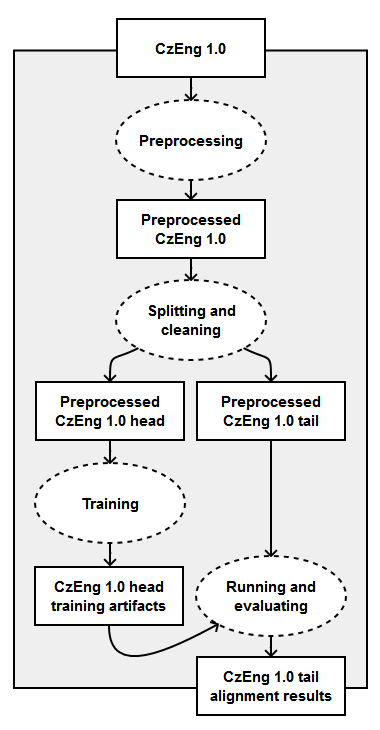
\includegraphics[width=0.50\textwidth]{images/czeng_experiment.png}
\end{figure}

\subsection{Preprocessing CzEng 1.0}
\label{subsection:czeng_experiment_preprocessing}

The entire CzEng 1.0 is preprocessed, as a whole. All the sequences of characters that are neither letters from any alphabet nor whitespaces nor even ASCII symbols are replaced with the Unicode symbol • (U+2022). Then, the corpus is tokenized and subsequently lowercased. The tokenization is done using MorphoDiTa (see Section~\ref{section:morphodita}). When running MorphoDiTa's script \texttt{run\_tokenizer} on the Czech and English parts of the parallel corpus, the argument \texttt{-{}-tokenizer} is set to \texttt{czech} and \texttt{english} respectively.

\subsection{Splitting and Cleaning CzEng 1.0}
\label{subsection:czeng_experiment_cleaning and splitting}

Preprocessed CzEng 1.0 is split horizontally exactly in half creating two separate parallel corpora, i.e.\ head and tail. The head is cleaned by excluding all pairs where either of the two sentences contains more than $50$ tokens ($286,318$ pairs are filtered out) or does not contain a single letter from any alphabet (more $103,251$ are discared). The tail is cleaned by only the latter of the two mentioned filters ($104,103$ pairs are exluded). The pairs containing overly long sentences are removed from the head to get better quality word alignment, which heavily affects the whole training process.

\subsection{Training Part I: Dictionary, Word Vectors}
\label{subsection:czeng_experiment_training_1}

As the first step of the training, SyMGIZA++ is applied (see Section~\ref{subsection:applying_symgiza}) to calculate the word alignment for the head. This includes the standard workflow with the scripts: \texttt{plain2snt}, \texttt{snt2cooc} and \texttt{mkcls}, where we request 2 optimization runs (\texttt{-n2}). For the execution of \texttt{symgiza}, we use the standard settings listed in Table~\ref{table:czeng_symgiza_settings}. From our experience, the method of final symmetrization yielding the best results is the ``union'' method (\texttt{-alig union}).
	
\begin{table}[!htb]
	\centering
	\caption{CzEng experiment: SyMGIZA++ settings}
	\label{table:czeng_symgiza_settings}
	\vspace{1em}
	\begin{tabular}{|l|l|}
		\hline
		\textbf{Description} & \textbf{Argument} \\
		\hline
		Number of threads & \texttt{-ncpus 4} \\
		Number of Model 1 iterations & \texttt{-m1 5} \\
		Number of Model 2 iterations & \texttt{-m2 5} \\
		Number of Model 3 iterations & \texttt{-m3 5} \\
		Number of Model 4 iterations & \texttt{-m4 5} \\
		Number of HMM iterations & \texttt{-mh 5} \\
		Dump Model 1 after 5\textsuperscript{th} iteration & \texttt{-t1} \\
		Dump Model 2 after 5\textsuperscript{th} iteration & \texttt{-t2} \\
		Dump Model 3, 4, 5 after 5\textsuperscript{th} iteration & \texttt{-t345} \\
		Dump Model HMM after 5\textsuperscript{th} iteration & \texttt{-th} \\
		Symmetrize Model 1 after 5\textsuperscript{th} iteration & \texttt{-m1symfrequency 5} \\
		Symmetrize Model 2 after 5\textsuperscript{th} iteration & \texttt{-m2symfrequency 5} \\
		Symmetrize Model 3, 4, 5 after 5\textsuperscript{th} iteration & \texttt{-m345symfrequency 5} \\
		Symmetrize Model HMM after 5\textsuperscript{th} iteration & \texttt{-mhsymfrequency 5} \\
		Symmetrization ``t'' tables multiplier & \texttt{-tm 2} \\
		Run final symmetrization & \texttt{-es 1} \\
		Use Union method in final symmetrization & \texttt{-alig union} \\
		Omit Diagonal option in final symmetrization & \texttt{-diagonal no} \\
		Omit Final option in final symmetrization & \texttt{-final no} \\
		Omit Both option in final symmetrization & \texttt{-both no} \\
		Probability for empty words & \texttt{-emprobforempty 0.0} \\
		Probability smoothing value & \texttt{-probsmooth 1e-7} \\
		\hline
	\end{tabular}
\end{table}

Subsequently, the bilingual dictionary is generated (see Section~\ref{subsection:generating_dictionary}) using the script \texttt{merge\_param.py}. The created dictionary contains $11,567,603$ entries.

Then, bivec is applied (see Section~\ref{subsection:applying_bivec}) to create the bilingual word vectors. Prior to the execution, the training dataset is preprocessed by replacing all the Unicode symbols • (U+2022) symbols with \texttt{<unk>} and the sequences consisting of numbers with zero symbol. We use the standard settings listed in Table~\ref{table:czeng_bivec_settings}. The resulting output contains $367,393$ vectors for the Czech and $179,869$ for the English part of the corpus.
	
\begin{table}[!htb]
	\centering
	\caption{CzEng experiment: bivec settings}
	\label{table:czeng_bivec_settings}
	\vspace{1em}
	\begin{tabular}{|l|l|}
		\hline
		\textbf{Description} & \textbf{Argument}\\
		\hline
		Language code of source language & \texttt{-src-lang en}\\
		Language code of target language & \texttt{-tgt-lang cs}\\
		Use the provided word alignment & \texttt{-align-opt 1}\\
		Cross-lingual learning rate multiplier & \texttt{-bi-weight 1.0}\\
		Use biskip model & \texttt{-cbow 0}\\
		Discard less appearing words & \texttt{-min-count 3}\\
		Size of the output vectors & \texttt{-size 40}\\
		Maximal skip length between words & \texttt{-window 5}\\
		Number of negative examples & \texttt{-negative 5}\\
		Save output in textual format & \texttt{-binary 0}\\
		Do not use hierarchical softmax & \texttt{-hs 0}\\
		Threshold for high-frequency source words & \texttt{-sample 1e-4}\\
		Threshold for high-frequency target words & \texttt{-tgt-sample 1e-4}\\
		Number of threads & \texttt{-threads 4}\\
		Do not evaluate results & \texttt{-eval 0}\\
		Number of iterations & \texttt{-iter 10}\\
		\hline
	\end{tabular}
\end{table}

\subsection{Training Part II: Classifier}
\label{subsection:czeng_experiment_training_2}

The pairs of parallel sentences from the head are distributed into artificial bins to form a supervised dataset for the training of the classifier (see Section~\ref{subsection:preparing_documents}). Each bin contains $50,000$ pairs of the parallel documents, i.e.\ $100,000$ individual documents. We consider this value to be an upper-bound estimate of an average number of paragraphs in either of the two languages located on an ordinary Czech--English web domain. The created dataset consists of $141$ bins. The last bin is an exception containing only $27,110$ pairs.

The document vectors are generated (see Section~\ref{subsection:generating_document_vectors}) using the script \texttt{create\_docvec.py}. The supervised dataset contains $7,027,110$ pairs of the parallel documents for which the script generates $6,467,817$ vectors for the Czech and $6,420,329$ vectors for the English documents. The numbers differ because the script discards duplicated documents within the bins.

The preliminary alignments are created (see Section~\ref{subsection:aligning_document_vectors}) running the script \texttt{align\_docvec.py}. For every Czech document a list of $20$ English candidate documents is created. Annoy (see Section~\ref{section:annoy}) is set to build search indices with $500$ trees and when performing a search it is requested to inspect $500 \times 20 \times 2 = 20,000$ nodes. These settings greatly affect the results. We follow the recommendations~\cite{annoy} to set the number of trees as large as possible given the amount of available memory and the number of nodes to be inspected as large as possible given the amount of available computational time.

The alignments are scored (see Section~\ref{subsection:scoring_alignments}) with the script \texttt{score\_align.py}. In this experiment, we use the expected ratio of the documents's lengths $\mu_{cs \rightarrow en} = 1.08$ with the standard deviation $\sigma_{cs \rightarrow en} = 0.28$. These values were estimated using the pairs of parallel sentences in the head.

The classifier is trained (see Section~\ref{subsection:training_binary_classifier}) with the script \texttt{train\_network.py}. The script creates the training dataset by randomly selecting approximately $20\%$ of all the available pairs of a Czech document with its top English candidate. Additionally, the selection contains nearly as many parallel pairs as non-parallel. The network model is provided by PyBrain (see Section~\ref{section:pybrain}). For completeness, let us describe its configuration; however, we shall not go into details~\cite{Sima96}. The network is a multilayer perceptron learning through the backwards error propagation. It has 4 input, 16 hidden and 2 output neurons. The input neurons are linear, the hidden layer uses sigmoid function and the output layer uses softmax function. The network is trained for $20$ epochs with the $1\%$ learning rate.

\subsection{Running}
\label{subsection:czeng_experiment_running}

The trained system is used to search for sentence pairs in the tail. The pairs of parallel sentences from the tail are distributed into artificial bins in a same manner as those from the head. Also, in this case, each bin contains $50,000$ pairs of the parallel documents, i.e.\ $100,000$ individual documents. In this scenario, each bin simulates a web domain with $50,000$ Czech and $50,000$ English paragraphs that we want to align. In contrast to real websites, these are perfectly parallel, all pages are available in both languages. This way, 147 bins are created. The last bin is an exception containing only $12,576$ pairs. For the purposes of the experiment, the original alignment of the tail is forgotten to not affect anyhow the evaluation process.

For the input dataset, the procedure follows with the exact same steps as for the supervised dataset in the second part of the training. Vectors are generated for all the documents. Using Annoy, the document vectors are aligned into preliminary alignments and these are subsequently scored. All of the settings remain unchanged. The input dataset consists of $7,312,576$ pairs for which $6,750,340$ vectors for the Czech and $6,703,831$ vectors for the English documents are generated. The differences between these numbers are caused again by the presence of duplicate documents within the bins.

In the last step, the trained binary classifier is applied  (see Section~\ref{subsection:applying_binary_classifier}) to obtain the refined alignments for the input dataset. This is done using the script \texttt{apply\_network.py}. The confidence threshold of the classifier is set to $50\%$. The refined alignments represent a subset of all the pairs of Czech documents with their top English candidates that the classifier accepts to be parallel.

\section{Experiment Results}
\label{section:czeng_experiment_results}

With the entire procedure of the experiment described, let us examine the results. The effectiveness of the method is measured after the individual steps of the aligning process. We present the results for the tail from the evaluation but also for the head from the second part of the training. This way we can compare the difference between the results when aligning the data used also in the first part of the training and the data not covered in the training.

Table~\ref{table:czeng_align} shows the quality of the preliminary alignments. The row with an index value $k$ shows how many times the parallel document ends up as a $k\textsuperscript{th}$ best candidate. The one with an index value $k \leq 20$ tells how many times the parallel document appears somewhere in the candidate list and the row with $k > 20$ shows how many times the parallel document is not in a candidate list at all. 

\begin{table}[!htb]
	\centering
	\caption{CzEng experiment: preliminary alignments}
	\label{table:czeng_align}
	\vspace{1em}
	\begin{tabular}{|r||r|r||r|r|}
		\hline
		& \multicolumn{2}{c||}{\textbf{Head (Training)}} & \multicolumn{2}{c|}{\textbf{Tail (Evaluation)}} \\
		\hline
		\textbf{Index} & \textbf{Count} & \textbf{Ratio (\%)} & \textbf{Count} & \textbf{Ratio (\%)} \\ \hline
		1 & 3,310,898 & 51.19 & 3,395,454 & 50.30 \\
		2 & 477,165 & 7.38 & 499,868 & 7.41 \\
		3 & 226,139 & 3.50 & 237,930 & 3.52 \\
		4 & 144,859 & 2.24 & 152,567 & 2.26 \\
		5 & 105,706 & 1.63 & 111,802 & 1.66 \\
		6 & 83,212 & 1.29 & 87,839 & 1.30 \\
		7 & 68,488 & 1.06 & 72,062 & 1.07 \\
		8 & 57,827 & 0.89 & 60,867 & 0.90 \\
		9 & 49,544 & 0.77 & 53,050 & 0.79 \\
		10 & 44,125 & 0.68 & 46,556 & 0.69 \\
		11 & 39,279 & 0.61 & 41,700 & 0.62 \\
		12 & 35,638 & 0.55 & 37,677 & 0.56 \\
		13 & 32,453 & 0.50 & 34,069 & 0.50 \\
		14 & 29,829 & 0.46 & 31,497 & 0.47 \\
		15 & 27,548 & 0.43 & 28,954 & 0.43 \\
		16 & 25,280 & 0.39 & 26,995 & 0.40 \\
		17 & 23,588 & 0.36 & 24,964 & 0.37 \\
		18 & 21,875 & 0.34 & 23,201 & 0.34 \\
		19 & 20,635 & 0.32 & 22,024 & 0.33 \\
		20 & 19,639 & 0.30 & 20,736 & 0.31 \\
		\hline
		$\leq 20$ & 4,843,727 & 74.89 & 5,009,812 & 74.22 \\
		$> 20$ & 1,624,090 & 25.11 & 1,740,528 & 25.78 \\
		\hline
		\textbf{Total} & 6,467,817 & 100.00 & 6,750,340 & 100.00 \\
		\hline
	\end{tabular}
\end{table}

The results for the head show, that $74.89\%$ Czech documents have their parallel English document included in the candidate list. This number is similar also for the tail, where it equals $74.22\%$. The difference is surprisingly small, as the training does not know anything about the tail. By further inspecting the results for the tail, we can observe, that of all the situations when the parallel document appears somewhere in the candidate list, in $67.78\%$ it is the top one and in $94.18\%$ it is included in the top $10$. This means that if we reduce the size of the search from $20$ to $10$, we can still expect approximately $69.89\%$ Czech documents to have the parallel English document somewhere in the candidate list. Reducing the size of the query increases the speed.

Table~\ref{table:czeng_align} shows the quality of the scored alignments. The process of scoring does not change the number of the Czech documents having a parallel English document present in the candidate list. Actually, it only reorders the candidate lists. The intention is to push the parallel documents within their candidate lists to the top as much as possible. The results show that the scoring function based on IBM Model 1 combined with the length comparison is effective. Again, the situation is obviously slightly better for the head. This is mainly caused by the fact, that the bilingual dictionary used in process is built-up from the head only. The results for the tail show that of all the times that parallel document appears in the candidate list, in $96.07\%$ it is the top one. We consider this a good reason why should the following process consider only the top candidates.

\begin{table}[!htb]
	\centering
	\caption{CzEng experiment: scored alignments}
	\label{table:czeng_score}
	\vspace{1em}
	\begin{tabular}{|r||r|r||r|r|}
		\hline
		& \multicolumn{2}{c||}{\textbf{Head (Training)}} & \multicolumn{2}{c|}{\textbf{Tail (Evaluation)}} \\
		\hline
		\textbf{Index} & \textbf{Count} & \textbf{Ratio (\%)} & \textbf{Count} & \textbf{Ratio (\%)} \\ \hline
		1 & 4,689,885 & 72.51 & 4,812,681 & 71.30 \\
		2 & 90,631 & 1.40 & 112,411 & 1.67 \\
		3 & 24,786 & 0.38 & 32,603 & 0.48 \\
		4 & 12,033 & 0.19 & 16,309 & 0.24 \\
		5 & 7,198 & 0.11 & 9,774 & 0.14 \\
		6 & 4,728 & 0.07 & 6,577 & 0.10 \\
		7 & 3,345 & 0.05 & 4,608 & 0.07 \\
		8 & 2,505 & 0.04 & 3,475 & 0.05 \\
		9 & 1,955 & 0.03 & 2,639 & 0.04 \\
		10 & 1,544 & 0.02 & 1,980 & 0.03 \\
		11 & 1,190 & 0.02 & 1,516 & 0.02 \\
		12 & 971 & 0.02 & 1,270 & 0.02 \\
		13 & 746 & 0.01 & 957 & 0.01 \\
		14 & 552 & 0.01 & 781 & 0.01 \\
		15 & 430 & 0.01 & 619 & 0.01 \\
		16 & 407 & 0.01 & 520 & 0.01 \\
		17 & 280 & 0.00 & 407 & 0.01 \\
		18 & 244 & 0.00 & 313 & 0.00 \\
		19 & 179 & 0.00 & 232 & 0.00 \\
		20 & 118 & 0.00 & 140 & 0.00 \\
		\hline
		$\leq 20$ & 4,843,727 & 74.89 & 5,009,812 & 74.22 \\
		$> 20$ & 1,624,090 & 25.11 & 1,740,528 & 25.78 \\
		\hline
		\textbf{Total} & 6,467,817 & 100.00 & 6,750,340 & 100.00 \\
		\hline
	\end{tabular}
\end{table}

The refined alignments are obtained with the $50\%$ confidence threshold. By gradually increasing the threshold and further filtering the alignments we measure the recall and the precision of the classifier at different confidence levels. The results are summarized in Table~\ref{table:czeng_refine}. The first column represents the confidence threshold. The second column represents the number of the document pairs correctly identified to be parallel, i.e.\ the number of true positives. The next column shows the number of false positives, which is the number of document pairs identified as parallel, but in fact they are not. The recall listed in the table is relative to the input of the classification process. The precision is the ratio of the true positives to all the positives. Figure~\ref{figure:czeng_classifier} shows how the recall and the precision change with respect to the confidence threshold of the classifier.

\begin{table}[!htb]
	\centering
	\caption{CzEng experiment: classifier effectiveness}
	\label{table:czeng_refine}
	\vspace{1em}
	\begin{tabular}{|r|r|r|r|r|}
		\hline
		\textbf{Conf.(\%)} & \textbf{True Pos.} & \textbf{False Pos.} & \textbf{Recall (\%)} & \textbf{Precision (\%)} \\ \hline
		50.00 & 4,254,069 & 284,174 & 88.39 & 93.74 \\
		55.00 & 4,179,076 & 248,921 & 86.83 & 94.38 \\
		60.00 & 4,095,812 & 217,081 & 85.10 & 94.97 \\
		65.00 & 4,000,964 & 188,595 & 83.13 & 95.50 \\
		70.00 & 3,892,099 & 162,537 & 80.87 & 95.99 \\
		75.00 & 3,761,728 & 138,619 & 78.16 & 96.45 \\
		80.00 & 3,599,299 & 114,985 & 74.79 & 96.90 \\
		85.00 & 3,385,007 & 89,813 & 70.34 & 97.42 \\
		90.00 & 3,073,706 & 64,730 & 63.87 & 97.94 \\
		95.00 & 2,621,246 & 46,522 & 54.47 & 98.26 \\
		99.00 & 1,808,067 & 23,028 & 37.57 & 98.74 \\
		\hline
	\end{tabular}
\end{table}

\begin{figure}[!htb]
	\centering
	\caption{CzEng experiment: classifier effectiveness}
	\label{figure:czeng_classifier}
	\vspace{1em}
	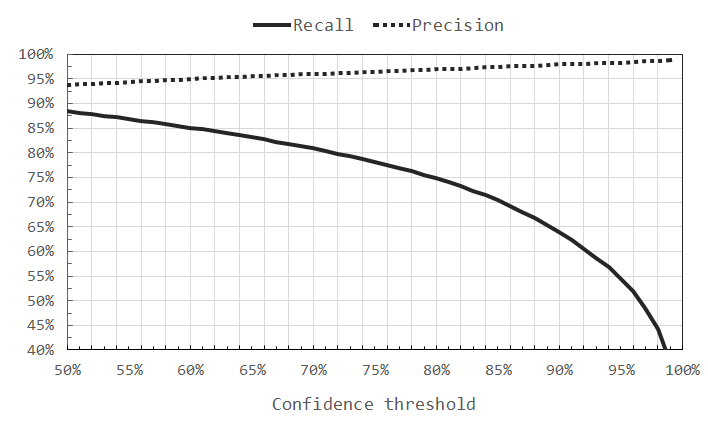
\includegraphics[width=1.00\textwidth]{images/czeng_classifier.png}
\end{figure}

The overall effectiveness of our method is listed in Table~\ref{table:czeng_overall}. These values are measured using the refined alignments without any form of additional filtering.

\begin{table}[!htb]
	\centering
	\caption{CzEng experiment: overall effectiveness}
	\label{table:czeng_overall}
	\vspace{1em}
	\begin{tabular}{|l|r|}
		\hline
		\textbf{Recall (\%)} & 63.02 \\
		\hline
		\textbf{Precision (\%)} & 93.74 \\
		\hline
	\end{tabular}
\end{table}

\section{Experiment Time Duration}
\label{section:czeng_experiment_duration}

The computer used for the experiment execution has Intel\textregistered{} Xeon\textregistered{} CPU E5-2630 v3 (20 MB Cache, 2.40 GHz) and 128 gigabytes (GB) of memory. Table~\ref{table:czeng_time_duration} lists the approximate time durations of the individual steps of the experiment.

\begin{table}[!htb]
	\centering
	\caption{CzEng experiment: time duration}
	\label{table:czeng_time_duration}
	\vspace{1em}
	\begin{tabular}{|l|r|}
		\hline
		\multicolumn{1}{|c|}{\textbf{Activity}} & \multicolumn{1}{c|}{\textbf{Duration (hh:mm)}} \\
		\hhline{|=|=|}
		\multicolumn{2}{|c|}{\textbf{Preprocessing}} \\
		\hline
		Tokenizing and lowercasing & 00:08 \\
		Splitting and cleaning & 00:05 \\
		\hline
		\multicolumn{2}{|c|}{\textbf{Training part I}} \\
		\hline
		Applying SyMGIZA++ & 13:21 \\
		Generating dictionary & 00:10 \\
		Applying bivec & 01:01 \\
		\hline
		\multicolumn{2}{|c|}{\textbf{Training part II}} \\ 
		\hline
		Generating document vectors & 00:37 \\
		Aligning document vectors (Annoy) & 05:52 \\
		Scoring alignments & 02:49 \\
		Training network classifier & 01:29 \\
		\hline
		\multicolumn{2}{|c|}{\textbf{Evaluation}} \\
		\hline
		Generating document vectors & 00:45 \\
		Aligning document vectors (Annoy) & 07:04 \\
		Scoring alignments & 04:10 \\
		Applying network classifier & 00:47 \\
		\hline
	\end{tabular}
\end{table}

\section{Extension: Lemmatization}
\label{section:czeng_experiment_extension}

As already noted (see Section~\ref{subsection:preprocessing_training_parallel_data}), we believe that preprocessing of both training and input data plays an important role in our method. The extension of the experiment described is this section is conducted with a goal to determine whether the lemmatization helps the method to achieve better quality results for the Czech--English language pair.

The procedure of the extended experiment is almost completely the same as in the original experiment. The only difference is in the preprocessing of the data. The lemmatization is added between the tokenization and lowercasing. The lemmatization is done with MorphoDiTa (see Section~\ref{section:morphodita}). When running the script \texttt{run\_tagger} on the Czech and English parts of the parallel corpus, it is provided with the models \texttt{czech-morfflex-pdt-131112.tagger-best\_accuracy}~\cite{Straka13} and \texttt{english-morphium-wsj-140407.tagger}~\cite{Straka14} respectively.

\begin{table}[!htb]
	\centering
	\caption{CzEng experiment (extended): scored alignments}
	\label{table:czeng_extended_score}
	\vspace{1em}
	\begin{tabular}{|r||r|r||r|r|}
		\hline
		& \multicolumn{2}{c||}{\textbf{Head (Training)}} & \multicolumn{2}{c|}{\textbf{Tail (Evaluation)}} \\
		\hline
		\textbf{Index} & \textbf{Count} & \textbf{Ratio (\%)} & \textbf{Count} & \textbf{Ratio (\%)} \\ \hline
		1 & 4,639,484 & 72.10 & 4,813,195 & 71.64 \\
		\vdots & \vdots & \vdots & \vdots & \vdots \\
		\hline
		$\leq 20$ &  4,813,165 & 74.80 & 5,022,948 & 74.76 \\
		$> 20$ & 1,621,610 & 25.20 & 1,695,537 & 25.24 \\
		\hline
		\textbf{Total} & 6,434,775 & 100.00 & 6,718,485 & 100.00 \\
		\hline
	\end{tabular}
\end{table}

With the lemmatization included, the dictionary built-up from the head contains only $6,225,379$ entries ($53.82\%$ of the original size). The extension also reduces the number of word vectors produced by bivec, which is  $173,861$ ($47.32\%$) vectors for the Czech and $163,993$ ($91.17\%$) for the English part of the corpus.

Table~\ref{table:czeng_extended_score} shows how the lemmatization affects the results. It shows the quality of the scored alignments. Although the table is not complete, it contains all the relevant data. The results show minimal improvement. For the tail, the amount of Czech documents having the parallel English document in the candidate list is increased by only $0.54\%$. Additionally, Table~\ref{table:czeng_extended_overall} lists the overall effectiveness of the method with lemmatization included. Again, the results are very similar.

\begin{table}[!htb]
	\centering
	\caption{CzEng experiment (extended): overall effectiveness}
	\label{table:czeng_extended_overall}
	\vspace{1em}
	\begin{tabular}{|l|r|}
		\hline
		\textbf{Recall (\%)} & 63.28 \\
		\hline
		\textbf{Precision (\%)} & 94.32 \\
		\hline
	\end{tabular}
\end{table}

Lemmatization can be thought of as a many-to-one mapping for words. By applying a transformation based on such a mapping we reduce the number of words within a corpus. With less words in the corpus, it is easier for the method to learn the associations between the words; however, the individual sentences are losing their contextual diversity. Apparently, the CzEng 1.0 data are already sufficiently large and the union word alignments do not benefit significantly from the denser statistics due to lemmatization.
